\subsubsubsection{Brisanje klijentskog naloga}

\begin{itemize}
    \item Kratak opis:
        \begin{itemize}
            \item Klijent briše svoj nalog i prestaje sa korišćenjem aplikacije.
        \end{itemize}
    \item Učesnici:
        \begin{itemize}
            \item Registrovani klijent ChooseFresh aplikacije.
        \end{itemize}
    \item Preduslovi:
        \begin{itemize}
            \item Klijent mora da bude prijavljen.
        \end{itemize}
    \item Postuslovi:
        \begin{itemize}
            \item Klijent je uspešno obrisao svoj nalog.
            \item Naplaćena su preostala dugovanja proistekla iz korišćenja aplikacije.
        \end{itemize}
    \item Osnovni tok:
        \begin{enumerate}
            \item Klijent pristupa veb stranici i otvara formu za brisanje naloga.
            \item Klijent unosi lozinku i potvrđuje da želi da obriše nalog.
            \item Sistem proverava tačnost podataka i vrši naplatu preostalih dugovanja.
            \item Sistem uklanja klijenta i sve njegove podatke iz sistema.
        \end{enumerate}
    \item Alternativni tok:
        \begin{itemize}
            \item[2.a] Klijent odustaje od brisanja naloga. Slučaj upotrebe se završava.
			\item[3.a] Ukoliko klijent ne unese validne podatke sistem ga obaveštava o greški prilikom brisanja. Slučaj upotrebe se nastavlja od koraka 2.
        \end{itemize}
\end{itemize}

\begin{figure}[H]
\begin{center}
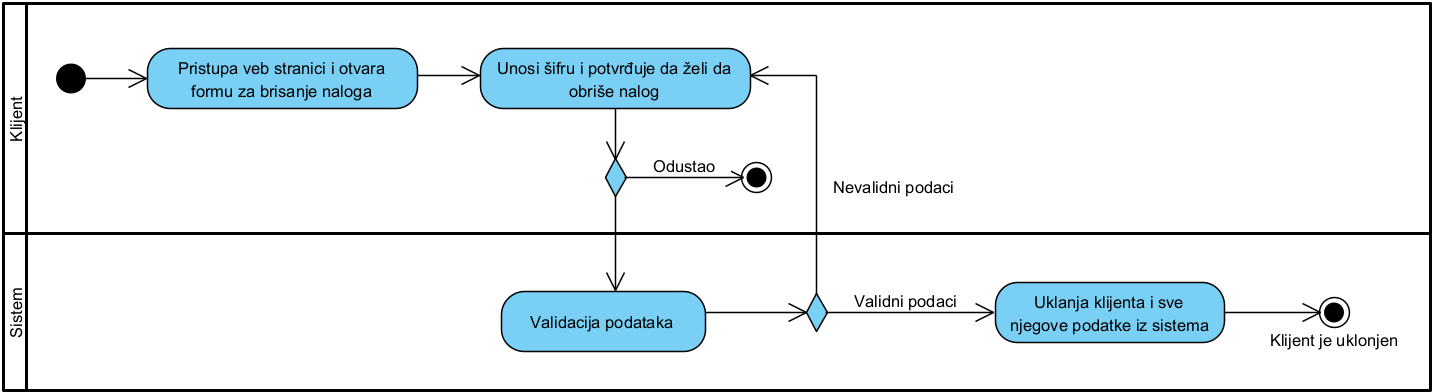
\includegraphics[width=\textwidth]{Pictures/activity_client_delete.png}
\end{center}
    \caption{Dijagram aktivnosti brisanja klijentskog naloga}
\label{fig:ActivityClientDelete}
\end{figure}
